\graphicspath{{3cyclic/asy/}}

\section{Cyclic \& Finite Abelian Groups}\label{chap:cyclic}

In this chapter we consider a general family of groups and see how to combine these to describe any finite abelian group.

\subsection{Definitions and Basic Examples}\label{sec:cycdef}

The foundational idea of a cyclic group is that it may be generated from a single element.

\begin{examples}{}{cyclicexmotiv}
	\exstart The integers $(\Z,+)$ are generated by the element 1: all integers may be produced by repeatedly combining 1 using only the group operation ($+$) and inverses ($-$). For instance,
	  \[
	  	-4=-(1+1+1+1)
	  \]
	\begin{enumerate}\setcounter{enumi}{1}
	  \item\label{ex:cyclicexmotiv2} The modular arithmetic groups $(\Z_n,+_n)$ (Section \ref{sec:modarith}) are also generated by (the remainder) 1. Since the group is finite, inverses are not necessary. For instance,
	  \[
	  	\Z_4=\{0,1,2,3\}=\{0,\ 1,\ 1+1,\ 1+1+1\}
	  \]
	 	\item The group $R_n$ of rotations of a regular $n$-gon (Definition \ref{defn:rot-dihedral}) is generated by the `1-step' rotation $\rho_1$: that is, $\rho_k=\rho_1^k$.
	\end{enumerate}
\end{examples}

We formalize this idea by considering the subset of a group that may be produced from a single element, the group operation, and inverses.

\begin{lemm}{Cyclic subgroup}{cyclicdef}
	Let $G$ be a group and $g\in G$. The set
	\[
		\ip{g}:=\{g^n:n\in\Z\}=\{\ldots,g^{-1},e,g,g^2,\ldots\}
	\]
	is a subgroup of $G$. We call this the \emph{cyclic subgroup\footnotemark{} generated by $g$.}
\end{lemm}

\footnotetext{%
	Since this is an abstract result, the lemma is written multiplicatively. If $G$ is an additive group, then cyclic subgroups are written $\ip{g}=\{ng:n\in\Z\}=\{\ldots,-2g,-g,0,g,2g,3g,\ldots\}$. As in Example \ref*{ex:cyclicexmotiv}.\ref{ex:cyclicexmotiv2}, for finite cyclic groups convention dictates that the identity element is written first, e.g.{} $\ip{g}=\{e,g,g^2,\ldots,g^{n-1}\}$. %
}

\begin{proof}
	We follow the subgroup criterion (Theorem \ref{thm:subgroup}).
	\begin{quote}
		\begin{description}
			\item[\emph{Non-emptiness}:] Plainly $g\in\ip g$.
			\item[\emph{Closure}:] Every element of $\ip g$ has the form $g^k$ for some $k\in \Z$. The required condition follows from standard exponential notation (Definition \ref{defn:assoc}): $g^k\cdot g^l=g^{k+l}\in\ip g$.
			\item[\emph{Inverses}:] This is Exercise \ref*{sec:groupaxioms}.\ref{exs:multinverse2}: $(g^k)^{-1}=g^{-k}\in\ip g$.
		\end{description}
	\end{quote}
	\vspace{-18pt}
\end{proof}

\begin{defn}{Cyclic group}{cyclic}
	A group $G$ is \emph{cyclic} if it has a \emph{generator}: $\exists g\in G$ such that $G=\ip g$.\smallbreak
	In any group $G$, the \emph{order of an element $g$} is the order (cardinality) of the cyclic subgroup $\ip g\le G$.
\end{defn}

\textcolor{red}{Warning!} Don't confuse the \emph{order of a group} $G$ with the \emph{order of an element} $g\in G$. Cyclic groups are precisely those containing elements (generators) whose order equals that of the group!


\goodbreak


\begin{examples*}{\ref{ex:cyclicexmotiv} cont}{}
	\exstart $\Z=\ip{1}=\ip{-1}$ is generated by either 1 or $-1$. The cyclic subgroup generated by 2 is the group of even numbers under addition
	\[
		\ip 2=\{\ldots,-2,0,2,4,\ldots\}=\{2m:m\in\Z\}=2\Z
	\]
	\begin{enumerate}\setcounter{enumi}{1}
	  \item $\Z_n$ is generated by both 1 and $-1=n-1$, but may have other generators (we'll consider how to find them all shortly). For instance, $\Z_5$ is generated also by 2:
	  \[
	  	\ip 2=\{2,\ 2+2,\ 2+2+2,\ \ldots\}=\{2, 4, 1, 3, 0\} =\Z_5
	  \]
		\item $R_n=\ip{\rho_1}=\{e,\rho_1,\rho_1^2,\ldots,\rho_1^{n-1}\}$. As with $\Z_n$, this group typically has other generators.
	\end{enumerate}
\end{examples*}

%\bigskip

%\boldsubsubsection{The Roots of Unity}

%For another family of cyclic groups, we consider subgroups of $(\C^\times,\cdot)$.

\begin{defn}{Roots of Unity}{}
	Let $n\in\N$. The group of \emph{$n\th$ roots of unity} $U_n$ is the cyclic subgroup of $(S^1,\cdot)$ generated by $\zeta:=e^{\frac{2\pi i}n}$:
	\[
		U_n:=\ip{\zeta}=\bigl\{1,\zeta,\zeta^2,\cdots,\zeta^{n-1}\bigr\}
	\]
	These are precisely the $n$ complex solutions to the equation $z^n=1$. To emphasize $n$, write $\zeta_n=\smash[t]{e^{\frac{2\pi i}n}}$. 
\end{defn}

\begin{minipage}[t]{0.75\linewidth}\vspace{-5pt}
	For instance $U_2=\ip{-1}=\{1,-1\}$ and $U_4=\ip{i}=\{1,i,-1,-i\}$. In general, the $n\th$ roots are the vertices of a regular $n$-gon centered at 0 with radius 1:
	\[
		\nm{\zeta^k}=\nm\zeta^k=1
		\quad\text{and}\quad
		\arg\zeta^k=\arg e^{\frac{2\pi k}{n}}=\tfrac{2\pi k}n=k\arg\zeta
	\]
	We stop listing the elements at $\zeta^{n-1}$ since $\zeta^n=e^{2\pi i}=1$. The periodicity of the complex exponential $(e^{i\theta}=1\Longleftrightarrow \theta\in 2\pi\Z)$ results in a simple tie-in with modular arithmetic:
	\[
		\zeta^k=\zeta^l\iff 1=\zeta^{k-l}=e^{\frac{2\pi i(k-l)}n}\iff k\equiv l\pmod n
	\]
\end{minipage}
\hfill
\begin{minipage}[t]{0.24\linewidth}\vspace{-5pt}
	\centering
	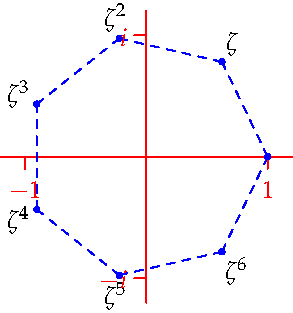
\includegraphics[scale=0.8]{cyclic-rootunity}\\
	Seventh roots: $\zeta_7=e^{\frac{2\pi i}7}$
\end{minipage}
\bigbreak

% 
% \begin{lemm}{}{}
% 	The $n\th$ roots of unity are precisely the $n$ (complex) roots of the equation $z^n=1$.\
% \end{lemm}
% 
% \begin{proof}
% 	Plainly $(\zeta^k)^n=(e^{\frac{2\pi ik}n})^n=e^{2\pi ik}=1$, so every element of $U_n$ solves $z^n=1$.\smallbreak
% 	For the converse, suppose $z^n=1$. Take the modulus to obtain $\nm{z}^n=1$. Since $\nm{z}$ is a non-negative real number, we see that $\nm{z}=1$, whence its polar form is $z=e^{i\theta}$. Now compute:
% 	\[
% 		1=z^n=(e^{i\theta})^n=e^{in\theta}\iff n\theta=2\pi k
% 	\]
% 	for some integer $k$ ($\ast$). But then $\theta=\frac{2\pi k}n$ and so
% 	\[
% 		z=e^{i\theta}=e^{\frac{2\pi i}nk}=\left(e^{\frac{2\pi i}n}\right)^k=\zeta^k\tag*{\qedhere}
% 	\]
% \end{proof}

\begin{examples}{}{unisoex}
	\exstart Observe that $\zeta_6^2=(e^{\frac{2\pi i}6})^2 =e^{\frac{2\pi i}3} =\zeta_3$.\par
	\begin{enumerate}\setcounter{enumi}{1}
		\begin{minipage}[t]{0.75\linewidth}\vspace{-8pt}
			\item[]This produces a subgroup relationship: writing $\textcolor{blue}{\zeta}=\zeta_6$, we have
			\[
				U_3 = \bigl\{\textcolor{red}{1},\textcolor{red}{\zeta^2},\textcolor{red}{\zeta^4}\bigr\}  < U_6 = \bigl\{\textcolor{red}{1},\textcolor{blue}{\zeta},\textcolor{red}{\zeta^2},\zeta^3,\textcolor{red}{\zeta^4},\zeta^5\bigr\}
			\]
			The picture makes this geometrically trivial (compare Example \ref*{ex:hexsubgroup}.\ref{ex:hexsubgroup2}).
		\end{minipage}
		\hfill
		\begin{minipage}[t]{0.24\linewidth}\vspace{-32pt}
			\flushright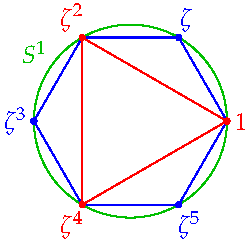
\includegraphics[scale=0.8]{cyclic-hexagon}
		\end{minipage}
	  
	  
	  \item\label{ex:unisoex2} (Example \ref{ex:z3r3iso}, cont.) \ Here is the Cayley table for $U_3$. Writing $1=\zeta^0$ and $\zeta=\zeta^1$ makes the relationship with $(\Z_3,+_3)$ and $(R_3,\circ)$ obvious:
		\[
			\def\arraystretch{1.1}
			\begin{array}{c||c|c|c}
				\cdot&1&\zeta&\zeta^2\\\hline\hline
				1&1&\zeta&\zeta^2\\\hline
				\zeta&\zeta&\zeta^2&1\\\hline
				\zeta^2&\zeta^2&1&\zeta
			\end{array}
			\qquad
			\begin{array}{c||c|c|c}
				\cdot&\zeta^{\textcolor{red}{0}}&\zeta^{\textcolor{blue}{1}}&\zeta^{\textcolor{Green}{2}}\\\hline\hline
				\zeta^{\textcolor{red}{0}}&\zeta^{\textcolor{red}{0}}&\zeta^{\textcolor{blue}{1}}&\zeta^{\textcolor{Green}{2}}\\\hline
				\zeta^{\textcolor{blue}{1}}&\zeta^{\textcolor{blue}{1}}&\zeta^{\textcolor{Green}{2}}&\zeta^{\textcolor{red}{0}}\\\hline
				\zeta^{\textcolor{Green}{2}}&\zeta^{\textcolor{Green}{2}}&\zeta^{\textcolor{red}{0}}&\zeta^{\textcolor{blue}{1}}
			\end{array}
			\qquad
			\begin{array}{c||c|c|c}
				+_3&\textcolor{red}{0}&\textcolor{blue}{1}&\textcolor{Green}{2}\\\hline\hline
				\textcolor{red}{0}&\textcolor{red}{0}&\textcolor{blue}{1}&\textcolor{Green}{2}\\\hline
				\textcolor{blue}{1}&\textcolor{blue}{1}&\textcolor{Green}{2}&\textcolor{red}{0}\\\hline
				\textcolor{Green}{2}&\textcolor{Green}{2}&\textcolor{red}{0}&\textcolor{blue}{1}
			\end{array}
			\qquad
			\begin{array}{c||c|c|c}
				\circ&\rho_{\textcolor{red}{0}}&\rho_{\textcolor{blue}{1}}&\rho_{\textcolor{Green}{2}}\\\hline\hline
				\rho_{\textcolor{red}{0}}&\rho_{\textcolor{red}{0}}&\rho_{\textcolor{blue}{1}}&\rho_{\textcolor{Green}{2}}\\\hline
				\rho_{\textcolor{blue}{1}}&\rho_{\textcolor{blue}{1}}&\rho_{\textcolor{Green}{2}}&\rho_{\textcolor{red}{0}}\\\hline
				\rho_{\textcolor{Green}{2}}&\rho_{\textcolor{Green}{2}}&\rho_{\textcolor{red}{0}}&\rho_{\textcolor{blue}{1}}
			\end{array}
		\]
		More formally, the three groups are \emph{isomorphic} $(U_3,\cdot)\cong (\Z_3,+_3)\cong (R_3,\circ)$. For a little practice here is a formal argument where we show that 
		\[
			\mu:\Z_3\to U_3:x\mapsto\zeta^x
		\]
		is an isomorphism. Since the domain $\Z_3$ consists of equivalence classes, we verify this carefully.
	\begin{description}
  	\item[\emph{Well-definition}:] If $x=y$ in $\Z_3$, then (as integers) $x=y+3n$ for some integer $n$. But then
  	\[
  		\mu(x) =\zeta^x =\zeta^{x+3n} =\zeta^y(\zeta^{3})^n =\zeta^y =\mu(y)
  	\]
  	\item[\emph{Homomorphism}:] $\mu(x+y) =\zeta^{x+y} =\zeta^x\zeta^y =\mu(x)\mu(y)$
  	\item[\emph{Injectivity}:] $\mu(x)=\mu(y)\Longrightarrow \zeta^x=\zeta^y\Longrightarrow \zeta^{x-y}=1\Longrightarrow x\equiv y\pmod 3\Longrightarrow x=y$ in $\Z_3$.
  	\item[\emph{Surjectivity}:] $\operatorname{range}\mu =\{\zeta^x:x\in\Z\} =\{1,\zeta,\zeta^2\} =U_3$, since $\zeta^{x+3n}=\zeta^x$.
	\end{description}
In the next section we'll essentially repeat this discussion in the abstract, so make sure this example makes sense before moving on.
	\end{enumerate}
\end{examples}



% 
% 
% The groups $\Z_n$ are typically those to which other cyclic groups are compared. Indeed in the next section we'll see that \emph{any} cyclic group of order $n$ is isomorphic to $\Z_n$!

% \begin{example}{}{}
% 	$(\Z_3,+_3)$ is isomorphic to the rotation group $(R_3,\circ)$ via $\phi(k)=\rho_{k\pmod 3}$.
% 	\smallbreak
% 	It is worth doing this slowly, since the domain is a set of equivalence classes:
% 	\begin{description}
% 		\item[\emph{Well-definition}:] If $y=x\in\Z_3$, then $y\equiv x\equiv r\pmod 3$ for some $r\in\{0,1,2\}$. But then
% 		\[
% 			\phi(y)=\rho_r=\phi(x)
% 		\]
% 		\item[\emph{Bijection}:] This is trivial $\phi:\{0,1,2\}\to\{\rho_0,\rho_1,\rho_2\}$.
% 		\item[\emph{Homomorphism}:] This is the formula for composition of rotations
% 		$\rho_k\rho_l=\rho_{k+l\negthickspace\pmod 3}$
% 	\end{description}
% \end{example}


\begin{exercises}
	Key concepts:\quad \emph{Generator\quad Order of an element\quad Cyclic (sub)group\quad Roots of unity}
	
	\begin{enumerate}	  
		\item Find/describe \emph{all} the generators of each cyclic group.
	  \begin{enumerate}
	      \item \makebox[120pt][l]{$(\Z,+)$ \hfill (b) }
	      $\{2^n3^{-n}:n\in\Z\}$ under multiplication
	      \setcounter{enumi}{2}
	      \item \makebox[120pt][l]{$(\Z_5,+_5)$ \hfill (d) }
	      $\left\{\begin{smatrix} a&0\\0&a \end{smatrix},\begin{smatrix} 0&b\\-b&0 \end{smatrix}: a,b=\pm 1\right\}$ under multiplication
	  \end{enumerate}
	  
	  
	  \item Compute the cyclic subgroup $\ip{12}$ of $\Z_{20}$.
	  
	  
	  \item Find all cyclic subgroups of $\Z_6$. What is the order of each element?
	  
	  
	  \item\label{exs:z5times2} Show that $\Z_5^\times=\{1,2,3,4\}$ forms a cyclic group under \emph{multiplication} modulo 5.
	
	
	  \item Recall Example \ref{ex:d3}. What is the cyclic subgroup of $D_3$ generated by $\rho_1$? Generated by $\mu_1$?
	  
	  
	  \item Find all cyclic subgroups of the Klein four-group. What is the order of each element?
	  
	  
	  \item Compute the cyclic subgroup $\ip{\zeta_8^5}$ of $U_8$, listing its elements in the order generated. 
	  	  
	  
		\item\begin{enumerate}
		  \item Prove that $(U_3,\cdot)$ is a subgroup of $(U_9,\cdot)$.
		  \item Complete the sentence and prove your assertion:
		  \begin{quote}
		  	$U_m\le U_n$ if and only if \underline{\qquad\scriptsize(relationship between $m$ and $n$)\qquad}
		  \end{quote}
		\end{enumerate}
	    	
	
	%   \item Define a binary relation on the half-open interval $[0,1)$ by
	%   \[x*y=x+y-\lfloor x+y\rfloor\]
	%   where $\lfloor x\rfloor$ is the floor (integer part) function. Thus $x*y$ is the \emph{fractional part} of $x+y$.
	%   \begin{enumerate}
	%     \item Let $S^1=\{z\in\C:\nm z=1\}$ be the unit circle in the complex plane. Find an isomorphism
	%   	\[\phi\bigl([0,1),*\bigr)\cong (S^1,\cdot)\]
	%   	and prove that it is such.
	%   	\item Prove or disprove: $([0,1),*)\cong(\R,+)$.\par
	%   (\emph{Hint: how many solutions has the equation $x*x=0$?})
	%   \end{enumerate}
	
		
		\item Modeling Example \ref*{ex:unisoex}.\ref{ex:unisoex2}, prove explicitly that $\Z_{197}\cong U_{197}$.
		
	  
	  \item Verify that $\phi:\C\to\C^\times:z\mapsto e^z$ is a homomorphism of abelian groups $(\C,+),(\C^\times,\cdot)$ but \emph{not} an isomorphism.\par
	  (\emph{This is in contrast to the real case: Example \ref*{ex:expiso}.\ref{ex:expiso1}})
		
		
		\item Give examples of:
		\begin{enumerate}
		  \item A \emph{finite} non-cyclic group.
		  \item An \emph{infinite} non-cyclic group.
		\end{enumerate}
		In both cases, explain how you know that your example is non-cyclic.
	 
	\end{enumerate}
\end{exercises}

\clearpage




\subsection{The Classification and Structure of Cyclic Groups}\label{sec:cyclicclass}

We describe all cyclic groups, their generators, and subgroup structures.

\begin{lemm}{}{}
	Every cyclic group is abelian.
\end{lemm}

\begin{proof}
	Let $G=\ip g$. Since any two elements of $G$ can be written $g^k,g^l$ for some $k,l\in\Z$, we see that
	\[
		g^kg^l=g^{k+l}=g^{l+k}=g^lg^k\tag*{\qedhere}
	\]
\end{proof}

The converse is \emph{false}: the Klein four-group $V$ is abelian but not cyclic (is the reason obvious to you?).\smallbreak

The next result is crucial to our classification; it is quite hard, so take your time and read carefully.


\begin{thm}{Isomorphs}{cyclicisomorph}
	Every cyclic group is isomorphic either to $(\Z,+)$ or to some $(\Z_n,+_n)$.\smallbreak
	If $G=\ip g$, then $\phi:x\mapsto g^x$ is an isomorphism $\phi:\Z_{(n)}\cong G$: ``map generator (1) to generator ($g$).''
\end{thm}

The proof is a little sneaky. To distinguish the two cases, we introduce a useful set of natural numbers $S:=\{m\in\N:g^m=e\}$ ($mg=e$ if $G$ is additive). To see why, consider a few examples of the theorem.

\begin{examples}{}{}
	\exstart If $G=R_3=\ip{\rho_1}$, then $\rho_1^m=e\iff 3\mid m$, whence $S=\{\textcolor{red}{3},6,9,\ldots\}$. Observe that $\textcolor{red}{3}=\min S$ is the \emph{order of $G$.} Moreover $\phi(x)=\rho_1^x$ is an isomorphism $\Z_3\cong R_4$ (Example \ref*{ex:unisoex}.\ref{ex:unisoex2}).
	\begin{enumerate}\setcounter{enumi}{1}
	  \item $\Z_4=\ip 1$ is additive, so $S=\{m\in\N:m=0\}=\{\textcolor{red}{4},8,12,\ldots\}$ \ (in $\Z_4$, $m=0$ means $4\mid m$!). Observe that $\textcolor{red}{4}=\min S$ is the order of $G=\nm{\Z_4}$.
	  \item $5\Z=\ip 5$ is an infinite cyclic group. In this case, $S=\{m\in\N:5m=0\}=\emptyset$ is \emph{empty}. This is isomorphic to $\Z$ via $\phi:\Z\to 5\Z:x\mapsto 5x$ (map the generator $1\in\Z$ to the generator $5\in 5\Z$).
	\end{enumerate}
\end{examples}

As the examples suggest, $S$ distinguishes the finite/infinite cases \emph{and} detects the order of $G$.

\begin{proof}
	\begin{description}\itemsep2pt
		\item[\normalfont If $S=\emptyset$:] Suppose $x>y$ and that $g^x=g^y$. Then $g^{x-y}=e\Longrightarrow x-y\in S$: contradiction. The elements $\ldots,g^{-2},g^{-1},e,g,g^2,\ldots$ are therefore \emph{distinct,} whence $\phi:\Z\to G:x\mapsto g^x$ is bijective.
		\item[\normalfont If $S\neq\emptyset$:] Let	$n=\min S$ and define $\phi:\Z_n\to G:x\mapsto g^x$. We first check this is well-defined:
		\begin{align*}
			y=x\in\Z_n&\implies y=x+kn\text{ for some $k\in\Z$}\\
			&\implies \phi(y)=g^y=\textcolor{red}{g^{x+kn}=g^x(g^n)^k=g^x}=\phi(x)
		\end{align*}
		Since the \textcolor{red}{highlighted} calculation is valid for all $x,k\in\Z$, we also conclude that
		\[
			G=\ip{g}\subseteq\{e,g,\ldots,g^{n-1}\} \tag{in particular, $G$ is \emph{finite}}
		\]
		Suppose two of these terms were equal; if $0\le y\le x\le n-1$, then
		\[
			g^x=g^y\implies g^{x-y}=e\implies x=y
		\]
		since $0\le x-y<n-1$ and $n=\min S$. Thus $n$ is the order of $G$ and $G=\{e,g,\ldots,g^{n-1}\}$.
	\end{description}\medskip
	In both cases, the homomorphism property is simply the exponential law
	\[
		\phi(x+y)=g^{x+y}=g^xg^y=\phi(x)\phi(y)\tag*{\qedhere}
	\]
\end{proof}


\begin{cor}{}{orderdefn}
	If the order of an \textbf{element} $g$ is finite, then it equals the minimal positive integer $n$ for which $g^n=e$. Moreover $g^m=e\Longleftrightarrow n\mid m$.
\end{cor}


\goodbreak

\begin{examples}{}{}
	\exstart The group of $7\th$ roots of unity $U_7$ is isomorphic to $\Z_7$ via $\phi:\Z_7\to U_7:k\mapsto \zeta_7^k$. As a sanity check, $7=\min\{m\in\N:\zeta_7^m=1\}$ is indeed the order of $\zeta_7$.
	\begin{enumerate}\setcounter{enumi}{1}
		\item Let $\xi=\smash[t]{e^{\frac{2\pi i}{\sqrt 2}}}$ and consider the cyclic subgroup $G:=\ip\xi<(\C^\times,\cdot)$. For integers $m$, observe that
		\[
			\xi^m=e^{\frac{2\pi im}{\sqrt 2}}=e=1\iff \tfrac m{\sqrt 2}\in\Z\iff m=0
		\]
		We conclude that $G$ is an \emph{infinite} cyclic group and that $\phi:\Z\to G:z\mapsto\xi^z$ is an isomorphism. We can interpret multiplication by $\xi$ as performing an irrational fraction $(\frac 1{\sqrt 2})$ of a full rotation.
		
		\item $(\R,+)$ is non-cyclic since its (uncountable) cardinality is larger than the (countable) cardinality of the integers. This is also straightforward to see directly: if $\R$ were cyclic with generator $x$, then we'd obtain an immediate contradiction
		\[
			\frac x2\notin\{\ldots,-2x,-x,0,x,2x,3x\ldots\}=\R\ni\frac x2
		\]
		The same argument shows that $(\Q,+)$ is not cyclic.
	\end{enumerate}
\end{examples}

\bigskip


All subgroups of a cyclic group may be straightforwardly described: they're also cyclic!

\begin{thm}{Subgroups of Cyclic Groups}{cyclic1}
	Any subgroup of a cyclic group is cyclic.
\end{thm}

The motivation for the proof is simple: the subgroup $2\Z\le\Z$ is generated by 2, the minimal \emph{positive} integer in the subgroup. Given a subgroup $H\le G$, we identify a suitable `minimal' element, and demonstrate that this generates $H$.

\begin{proof}
	Suppose $H\le G=\ip g$. If $H=\{e\}$ is trivial, we are done: $H$ is cyclic!\smallbreak
	Otherwise, $\exists s\in\N$ minimal so that $g^s\in H$. We claim that $H$ is generated by $g^s$.
	\begin{description}\itemsep0pt
		\item[$\bigl(\ip{g^s}\subseteq H\bigr)$] This is trivial since $g^s\in H$.
		\item[$\bigl(H\subseteq \ip{g^s}\bigr)$] Let $g^m\in H$. By the division algorithm, there exist unique integers $q,r$ such that
		\[
			m=qs+r\quad\text{and}\quad 0\le r<s
		\]
		But then, since $H$ is closed under $\cdot$ and inverses,
		\[
			g^m=g^{qs+r}=(g^s)^qg^r\implies g^r=(g^s)^{-q}g^m\in H \tag{$\ast$}
		\]
		The minimality of $s$ now forces $r=0$, from which we conclude that $g^m=(g^s)^q\in\ip{g^s}$.\qedhere 
	\end{description}
\end{proof}

If the proof seems too hard to follow, try rewriting it carefully when $G=\Z$, $H=2\Z$ and $s=2$: remember that $G$ is \emph{additive}, so ($\ast$) simply becomes $r=-2s+m\in H$, from which $m=2s$\ldots


\goodbreak

We treat the finite and infinite cases separately. The infinite case is very simple.

\begin{cor}{Subgroups of infinite cyclic groups}{infcyclic}
	If $G$ is an infinite cyclic group and $H\le G$, then either $H=\{e\}$ is trivial, or $H\cong G$.
\end{cor}

We leave the proof as an exercise (just generalize the following example!).

\begin{example}{}{}
	It is helpful to write things out explicitly in additive notation when $G=\Z$. Since every subgroup is cyclic, there are two cases:
	\begin{itemize}\itemsep2pt
	  \item The trivial subgroup: $\ip 0=\{0\}$.
	  \item Every other subgroup: $\ip{s}=s\Z$ when $s\neq 0$. Each of these is isomorphic to $\Z$ via an isomorphism $\phi:\Z\to s\Z:x\mapsto sx$.
	\end{itemize}
\end{example}


\smallskip


\emph{Finite} cyclic groups are a little more complicated so we first consider an example.

\begin{example}{}{}
	Consider $U_6=\{1,\zeta,\zeta^2,\zeta^3,\zeta^4,\zeta^5\}$ under multiplication. Since all subgroups are cyclic, we need only consider the subgroup $\ip x$ generated by each element $x$.
	\[
		\makebox[230pt][l]{%
			$\def\arraystretch{1.05}
			\begin{array}[t]{l|c}
				x & \text{subgroup}\ip x\\ \hline
				1 & \{1 \} \\
				\textcolor{red}{\zeta} & \textcolor{red}{\{1,\zeta,\zeta^2,\zeta^3,\zeta^4,\zeta^5\}}\\
				\textcolor{blue}{\zeta^2} & \textcolor{blue}{\{1,\zeta^2,\zeta^4\}}\\
				\textcolor{Green}{\zeta^3} & \textcolor{Green}{\{1,\zeta^3\}}\\
				\textcolor{blue}{\zeta^4} & \textcolor{blue}{\{1,\zeta^4,\zeta^2\}}\\
				\textcolor{red}{\zeta^5} & \textcolor{red}{\{1,\zeta^5,\zeta^4,\zeta^3,\zeta^2,\zeta\}}
			\end{array}$
		}
		\makebox[0pt][c]{%
			$\xymatrix @C0pt @R24pt{%
				& \textcolor{red}{\ip{\zeta}}=U_6 \ar@{-}[dl] \ar@{-}[dr] & \\
				\textcolor{blue}{\ip{\zeta^2}}=U_3 \ar@{-}[dr] & & \textcolor{Green}{\ip{\zeta^3}}=U_2 \ar@{-}[dl] \\
				& \ip{1}=U_1 &
			}$
		}
	\]
	Observe the repetitions: $\ip{\textcolor{red}{\zeta}}=\ip{\textcolor{red}{\zeta^5}}=U_6$ and $\ip{\textcolor{blue}{\zeta^2}}=\ip{\textcolor{blue}{\zeta^4}}=U_3$.
	\smallbreak
	For comparison, here is the same data for subgroups of the additive group $(\Z_6,+_6)$.
	\[
		\makebox[230pt][l]{%
			$\def\arraystretch{1.05}
			\begin{array}[t]{l|c}
				x & \text{subgroup}\ip x\\ \hline
				0 & \{0\} \\
				\textcolor{red}{1} & \textcolor{red}{\{0,1,2,3,4,5\}}\\
				\textcolor{blue}{2} & \textcolor{blue}{\{0,2,4\}}\\
				\textcolor{Green}{3} & \textcolor{Green}{\{0,3\}}\\
				\textcolor{blue}{4} & \textcolor{blue}{\{0,4,2\}}\\
				\textcolor{red}{5} & \textcolor{red}{\{0,5,4,3,2,1\}}
			\end{array}$
		}
	\makebox[0pt][c]{%
		$\xymatrix @C0pt @R24pt{%
			& \textcolor{red}{\ip{1}}=\Z_6 \ar@{-}[dl] \ar@{-}[dr] & \\
			\textcolor{blue}{\ip{2}}\cong\Z_3 \ar@{-}[dr] & & \textcolor{Green}{\ip{3}}\cong\Z_2 \ar@{-}[dl] \\
			& \ip{0}\cong\Z_1 &
			}$
		}
	\]
	As must be since the groups are isomorphic, the difference is entirely notational! One subtle difference is that we don't use \emph{equals} in the second subgroup diagram: for instance, $\textcolor{blue}{\ip{2}}=\{0,2,4\}$ is \emph{isomorphic} but \emph{not equal} to $\Z_3=\{0,1,2\}$.
\end{example}

You should be able to guess two patterns from the example:
\begin{itemize}\itemsep2pt
	\item $\Z_n$ has exactly one subgroup of order $d$ for each divisor $d$ of $n$.
	\item If $d\in\Z_n$ is a divisor of $n$, then $\ip{d}\cong \Z_{\frac nd}$.
\end{itemize}
The next result merely asserts these patterns for general finite cyclic $G$.

\goodbreak

\begin{cor}{Subgroups of finite cyclic groups}{subscyclic}
	Let $G=\ip g$ have order $n$. Then $G$ has a \textbf{unique subgroup} of each order dividing $n$. More precisely, 
	\[
		d=\gcd(s,n)\Longrightarrow \ip{g^s}=\langle{g^d}\rangle, \quad\text{where this subgroup has order $\tfrac nd$}
	\]
	In particular, $g^s$ is a generator of $G$ if and only if $\gcd(s,n)=1$.
\end{cor}


\begin{proof}
	Suppose $d=\gcd(s,n)$. We prove set inclusion in both directions.
	\begin{description}
		\item[$(\subseteq)$] Since $d$ divides $s$ we have $s=kd$ for some $k\in\Z$, and so
		\[
			g^s=(g^d)^{k}\in\bigl\langle g^d\big\rangle \implies (g^s)^t=(g^d)^{kt}\implies  \ip{g^s}\subseteq\bigl\langle g^d\big\rangle
		\]
		\item[$(\supseteq)$] Apply Bézout's identity (extended Euclidean alg.): $d=\kappa s+\lambda n$ for some $\kappa,\lambda\in\Z$, whence
		\[
			g^d=(g^s)^\kappa (g^n)^\lambda=(g^s)^\kappa\in\ip{g^s} \implies \bigl\langle g^d\big\rangle\subseteq\ip{g^s}
		\]
	\end{description}
	To finish, consider the elements in $\langle{g^d}\rangle$. Since $d\mid n$, there are precisely $\frac nd$ of these, specifically
	\[
		\langle{g^d}\rangle=\bigl\{e,g^d,g^{2d},\ldots,g^{n-d}\bigr\}\tag*{\qedhere}
	\]
\end{proof}


As before, the result is worth restating for the additive group $(\Z_n,+_n)$:
\[
	\tcbhighmath{d=\gcd(s,n)\Longrightarrow \ip s=\ip d\cong\Z_{\frac nd},
	\quad\text{in particular, $s$ generates $\Z_n$}\Longleftrightarrow \gcd(s,n)=1}
\]



\begin{example}{}{}
% \begin{enumerate}
%   \begin{minipage}[t]{0.85\linewidth}\vspace{0pt}
%   \item $\Z_8$ is generated by $1,3,5$ and $7$, since these are precisely the elements $s\in\Z_8$ for which $\gcd(s,8)=1$. For example,
%   \[\Z_8=\ip 5=\{5,2,7,4,1,6,3,0\}\cong C_{\frac 8{\gcd(5,8)}}\]
%   The subgroup generated by 6 is
%   \[\ip 6=\{6,4,2,0\}\]
%   which has order $4=\frac 8{\gcd(6,8)}$ in accordance with the Theorem. This subgroup is also generated by 2. The complete collection of subgroups and their generators is shown in the table, and the subgroup diagram is also drawn.
%   \[\begin{array}{l|c|c|c}
%     x & \gcd(x,8) & \quotient{8}{\gcd(x,8)} & \text{subgroup generated }\ip x\\ \hline
% 0(8) & 0(8)  & 1 & C_1\\
% 4 & 4 & 2 & C_2\\
% 2,6 & 2 & 4 & C_4\\
% 1,3,5,7 & 1 & 8 & \Z_8\\
%     \end{array}\]
%   \end{minipage}\begin{minipage}[t]{0.15\linewidth}\vspace{60pt}
%     \[ \xymatrix{\Z_{8}=\ip{1} \ar@{-}[d]\\
% C_{4}\cong\ip 2 \ar@{-}[d]\\
% C_2\cong\ip 4 \ar@{-}[d]\\
% C_1\cong\ip 0}\]
%   \end{minipage}
We describe the subgroups of $\Z_{30}$ and construct its subgroup diagram. The first column lists each divisor $d$ of $30$ (the possible values of $\gcd(\textcolor{red}{x},30)$), the second column the isomorphic group $\Z_{\frac{30}d}$, and the third the subgroup generated by each value $\textcolor{red}{x}\in\Z_{30}$.
  \[
  	\def\arraystretch{1.05}
  	\begin{array}[t]{c|c|c}
			d=\gcd(\textcolor{red}{x},30) & \text{Isomorph }\Z_{\frac{30}d} & \text{Subgroup } \ip{\textcolor{red}{x}} \\\hline
			1 & \Z_{30} & \{0,\textcolor{red}{1},2,3,\ldots,\textcolor{red}{7},\ldots,\textcolor{red}{11},12,\textcolor{red}{13},\ldots,\textcolor{red}{17},18,\textcolor{red}{19},\ldots,\textcolor{red}{23},\ldots,\textcolor{red}{29}\}\\
			2 & \Z_{15} & \{0,\textcolor{red}{2},\textcolor{red}{4},6,\textcolor{red}{8},10,12,\textcolor{red}{14},\textcolor{red}{16},18,20,\textcolor{red}{22},24,\textcolor{red}{26},\textcolor{red}{28}\}\\
			3 & \Z_{10} & \{0,\textcolor{red}{3},6,\textcolor{red}{9},12,15,18,\textcolor{red}{21},24,\textcolor{red}{27}\}\\
			5 & \Z_6 & \{0,\textcolor{red}{5},10,15,20,\textcolor{red}{25}\}\\
			6 & \Z_5 & \{0,\textcolor{red}{6},\textcolor{red}{12},\textcolor{red}{18},\textcolor{red}{24}\}\\
			10 & \Z_3 & \{0,\textcolor{red}{10},\textcolor{red}{20}\}\\
			15 & \Z_2 & \{0,\textcolor{red}{15}\}\\
			0\,(30) & \Z_1 & \{\textcolor{red}{0}\}
   \end{array}
  \]
    
	\begin{minipage}[t]{0.62\linewidth}\vspace{0pt}
		The generators of each subgroup are \textcolor{red}{red} in the table. In the subgroup diagram, the obvious generator is given for each.\smallbreak
		The \emph{shape} of the subgroup diagram (this one looks something like a cube) depends on the fact that in the \emph{prime decomposition} $30=2\cdot 3\cdot 5$, each prime appears \emph{exactly once}.
	\end{minipage}
	\hfill
	\begin{minipage}[t]{0.36\linewidth}\vspace{-5pt}
		\flushright%
		$\xymatrix @C4pt @R11pt{%
		 	& \ip{1}=\Z_{30} \ar@{-}[dl] \ar@{-}[d] \ar@{-}[dr] & \\
			\ip{2}\cong \Z_{15} \ar@{-}[d] \ar@{-}[dr] & \ip{3}\cong\Z_{10} \ar@{-}[dl] \ar@{-}[dr] & \ip{5}\cong\Z_6 \ar@{-}[d] \ar@{-}[dl] \\
			\ip{6}\cong\Z_5 \ar@{-}[dr] & \ip{10}\cong \Z_{3} \ar@{-}[d] & \ip{15}\cong\Z_2 \ar@{-}[dl] \\
 & \ip{0}\cong\Z_1 &}$
	\end{minipage}
 
\end{example}

\goodbreak

\begin{exercises}
	Key concepts:\quad \emph{Every cyclic group isomorphic to $\Z$ or $\Z_n$}
	\begin{quote}
		\emph{$\ip g$ order $n\implies \ip{g^s}$ order $\frac n{\gcd(s,n)}$\qquad Subgroup diagrams for finite cyclic groups}
	\end{quote}
	
	
	\begin{enumerate}
		\item Construct the subgroup diagram and give a generator of each subgroup:
		\begin{enumerate}
		  \item $(\Z_{10},+_{10})$\qquad\qquad (b)\lstsp $(\Z_{42},+_{42})$.
		\end{enumerate}
	  
	  
	  \item A generator of the cyclic group $U_n$ group is known as a \emph{primitive $n\th$ root of unity.} For instance, the primitive 4\th\ roots are $\pm i$. Find all the primitive roots when:
	  \begin{enumerate}
	    \item $n=5$\hfill (b)\lstsp $n=6$\hfill (c)\lstsp $n=8$\hfill (d)\lstsp $n=15$\hspace*{\fill}\hspace*{\fill}
	  \end{enumerate}
		
		
		\item Find the complete subgroup diagram of $U_{p^2q}$ where $p,q$ are distinct primes.\par
		(\emph{Hint: Try $U_{12}$ first if this seems too difficult})
	  
	  
	  \item If $r\in\N$ and $p$ is prime, find all subgroups of $(\Z_{p^r},+_{p^r})$ and give a generator for each.
		
		
	  \item\begin{enumerate}
	    \item Suppose $\phi:G\to H$ is an isomorphism of cyclic groups. If $g$ is a generator of $G$, prove that $\phi(g)$ is a generator of $H$. Do you really need $\phi$ to be an \emph{isomorphism} here?
	  
	  	\item If $G$ is an infinite cyclic group, how many generators has it?
	  	
			\item Recall Exercise \ref*{sec:cycdef}.\ref{exs:z5times}. Describe an isomorphism $\phi:\Z_4\to\Z_5^\times$.
	  \end{enumerate} 
	  
	  
	  \item True or false: In \emph{any} group $G$, if $g$ has order $n$, then $g^s$ has order $\frac n{\gcd(s,n)}$. Explain.
	  
	  
	  \item Suppose $G=\ip g$ is infinite and $H=\ip{g^s}$ is an infinite subgroup. Prove Corollary \ref{cor:infcyclic} by explicitly finding an isomorphism $\phi:G\to H$.
	
	
	  \item Prove Corollary \ref{cor:orderdefn}: you'll need the division algorithm for the second part!
	  
	  
		\item Let $x,y$ be elements of a group $G$. If $xy$ has finite order $n$, prove that $yx$ also has order $n$.\par
		(\emph{Hint: $(xy)^m=x(yx)^{m-1}y$})
		
		
% 		\item\label{exs:znmult} Let $\Z_n^\times=\bigl\{x\in\Z_n:\gcd(x,n)=1\bigr\}$ be the set of generators of the additive group $(\Z_n,+_n)$. Prove that $\Z_n^\times$ is a group under \emph{multiplication} modulo $n$.\par
% 		(\emph{Hint: Use Bézout's identity (extended Euclidean Algorithm)})
		
	%   
	%   \item Which of the following sets generate the group $(\Z_{30},+_{30})$? For those sets that do not generate the group give the subgroup that they do generate.
	%   \begin{enumerate}
	%       \item $\{2\}$
	%       \item $\{2,6\}$
	%       \item $\{2,3\}$
	%       \item $\{7\}$
	%       \item $\{12,18\}$
	%       \item $\{6,15\}$
	%   \end{enumerate}
		
		
		\item\label{exs:finitegen} Let $G$ be a group and $X$ a non-empty subset of $G$. The \emph{subgroup generated by $X$} is the subgroup created by making all possible combinations of elements and inverses of elements in $X$.
		\begin{enumerate}
		  \item Explain why $(\Z,+)$ is generated by the set $X=\{2,3\}$.
		  \item If $m,n\in(\Z,+)$, show $X=\{m,n\}$ generates $d\Z$, where $d=\gcd(m,n)$.
		  \item The Klein four-group $V$ is not cyclic, so it cannot be generated by a singleton set. Find a set of \emph{two} elements which generates $V$.
		  \item Describe the subgroup of $(\Q,+)$ generated by $X=\{\frac 12,\frac 13\}$.
		  \item (Hard) \ $(\Q,+)$ is plainly generated by the \emph{infinite} set $\{\frac 1n:n\in\N\}$. Explain why $(\Q,+)$ is \emph{not finitely generated}: i.e.\ there exists no \emph{finite} set $X$ generating $\Q$.\par
		  (\emph{Hint: Think about the prime factors of the denominators of elements of $X$})
		\end{enumerate}

	
	\end{enumerate}
\end{exercises}



\subsection{Direct Products \& Finite Abelian Groups}\label{sec:direct}


In this section we discuss a straightforward way to create new groups from old using the \emph{Cartesian product.}

\begin{example}{}{}
	Given $\Z_2=\{0,1\}$, the Cartesian product
	\[
		\Z_2\times \Z_2=\bigl\{(0,0),(0,1),(1,0),(1,1)\bigr\}
	\]
	has \emph{four} elements. This set has a natural group structure by via addition of co-ordinates
	\[
		(x,y)+(v,w):=(x+v,y+w)
	\]
	where $x+v$ and $y+w$ are both computed in $(\Z_2,+_2)$. This is a binary operation on $\Z_2\times\Z_2$, with a familiar-looking Cayley table: it has exactly the same structure as the Klein four-group!
	\begin{quote}
		\scalebox{1}{$%
			\begin{array}{c||c|c|c|c}
				+ & (0,0) & \textcolor{Green}{(0,1)} & \textcolor{red}{(1,0)} & \textcolor{blue}{(1,1)}\\\hline\hline
				(0,0) & (0,0) & \textcolor{Green}{(0,1)} & \textcolor{red}{(1,0)} & \textcolor{blue}{(1,1)}\\\hline
				\textcolor{Green}{(0,1)} & \textcolor{Green}{(0,1)} & (0,0) & \textcolor{blue}{(1,1)} & \textcolor{red}{(1,0)}\\\hline
				\textcolor{red}{(1,0)} & \textcolor{red}{(1,0)} & \textcolor{blue}{(1,1)} & (0,0) & \textcolor{Green}{(0,1)}\\\hline
				\textcolor{blue}{(1,1)} & \textcolor{blue}{(1,1)} & \textcolor{red}{(1,0)} & \textcolor{Green}{(0,1)} & (0,0)
			\end{array}%
		$}
		\qquad\scalebox{1.5}{$\leftrightsquigarrow$}\qquad
		\scalebox{1}{$%
			\begin{array}{c||c|c|c|c}
				\circ & e & \textcolor{Green}{a} & \textcolor{red}{b} & \textcolor{blue}{c}\\\hline\hline
				e & e & \textcolor{Green}{a} & \textcolor{red}{b} & \textcolor{blue}{c}\\\hline
				\textcolor{Green}{a} & \textcolor{Green}{a} & e & \textcolor{blue}{c} & \textcolor{red}{b}\\\hline
				\textcolor{red}{b} & \textcolor{red}{b} & \textcolor{blue}{c} & e & \textcolor{Green}{a}\\\hline
				\textcolor{blue}{c} & \textcolor{blue}{c} & \textcolor{red}{b} & \textcolor{Green}{a} & e
			\end{array}%
		$}
	\end{quote}
	We conclude that $\Z_2\times\Z_2\cong V$ is indeed a group.
\end{example}


This construction works in general.

\begin{thm}{Direct product}{directprod}
	The natural component-wise operation on the Cartesian product
	\[
		\smash[t]{\prod\limits_{k=1}^n} G_k=G_1\times\cdots\times G_n,\qquad (x_1,\ldots,x_n)\cdot(y_1,\ldots,y_n):=(x_1y_1,\ldots,x_ny_n)
	\]
	defines a group structure: the \emph{direct product.} This group is abelian if and only if each $G_k$ is abelian.
\end{thm}

The proof is a simple exercise. Being a Cartesian product, a direct product has order equal to the product of the orders of its components
\[
	\nm{\prod\limits_{k=1}^n G_k}=\prod\limits_{k=1}^n\nm{G_k}
\]
\vspace{2pt}


\begin{examples}{}{direct1}
	\exstart The direct product of the groups $(\Z_2,+_2)$ and $(\Z_3,+_3)$ is
	\[
		\Z_2\times\Z_3=\bigl\{(0,0),(0,1),(0,2),(1,0),(1,1),(1,2)\bigr\}
	\]
	This is abelian of order 6, so we might guess it to be isomorphic to $(\Z_6,+_6)$ and thus cyclic. This is indeed the case: simply observe that $(1,1)$ is a generator,
	\[
		\ip{(1,1)}=\bigl\{(1,1),(0,2),(1,0),(0,1),(1,2),(0,0)\bigr\}=\Z_2\times\Z_3
	\]
	The map $\phi(x)=(x,x)$ is therefore an isomorphism $\phi:\Z_6\cong\Z_2\times \Z_3$.

	\goodbreak

	\begin{enumerate}\setcounter{enumi}{1}
	% \item As observed above, $\Z_2\times\Z_2=\{(0,0),(0,1),(1,0),(1,1)\}$. is isomorphic to the Klein 4-group.
		\item If each $G_k$ is \emph{abelian} and \emph{written additively,} the direct product can instead be called the \emph{direct sum}
		\[
			\bigoplus_{k=1}^nG_k=G_1\oplus\cdots\oplus G_n
		\]
		We won't use this notation,\footnotemark\ though you've likely encountered it in linear algebra: the direct sum of $n$ copies of the real line $\R$ is the familiar vector space
		\[
			\R^n=\bigoplus_{i=1}^n\R=\R\oplus\cdots\oplus\R
		\]
	\end{enumerate}
\end{examples}

\footnotetext{%
	In these notes a direct product/sum will only ever have \emph{finitely many} terms, in which case the concepts are identical. As you can read elsewhere, when there are infinitely many factors, the concepts are slightly different.%
}


\boldsubsubsection{Orders of Elements in a Direct Product}

In Example \ref{ex:direct1}.1, we saw that the element $(1,1)\in\Z_2\times\Z_3$ had order 6 and thus generated the group. To help spot the pattern, consider another example.

\begin{example}{}{}
	What is the order of the element $(10,2)\in\Z_{12}\times \Z_8$? Recall Corollary \ref{cor:subscyclic}:
	\begin{itemize}\itemsep0pt
	  \item $10\in\Z_{12}$ has order $6=\frac{12}{\gcd(10,12)}$
	  \item $2\in\Z_8$ has order $4=\frac 8{\gcd(2,8)}$
	\end{itemize}
	If we repeatedly add $(10,2)$ to itself, then the \textcolor{red}{first co-ordinate resets after 6} summations, while the \textcolor{blue}{second resets after 4}. For \emph{both} to reset simultaneously, we need a \emph{common multiple} of \textcolor{red}{6} and \textcolor{blue}{4} summands. We can check this explicitly:
	\[
		\bigl\langle(10,2)\bigr\rangle = \bigl\{(10,2), (8,4), (6,6), (4,\textcolor{blue}{0}), (2,2), (\textcolor{red}{0},4), (10,6), (8,\textcolor{blue}{0}), (6,2), (4,4), (2,6), (\textcolor{red}{0},\textcolor{blue}{0})\bigr\}
	\]
	The order of the element $(10,2)$ is indeed the \emph{least common multiple} $12=\lcm(6,4)$.
\end{example}


\begin{thm}{}{directorder}
	Suppose $x_k\in G_k$ has order $r_k$. Then $(x_1,\ldots,x_n)\in \prod\limits_{k=1}^n G_k$ has order $\lcm(r_1,\ldots,r_n)$.
\end{thm}

\begin{proof}
	Simply appeal to Corollary \ref{cor:orderdefn}:
	\[
		(x_1,\ldots,x_n)^m=(x_1^m,\ldots,x_n^m)=(e_1,e_2,\ldots,e_n)\iff \forall k,\ x_k^m=e_k \iff \forall k,\ r_k\mid m
	\]
	The order is the minimal positive integer $m$ satisfying this, namely $m=\lcm(r_1,\ldots,r_n)$.
\end{proof}



\begin{example}{}{prodorder}
	Find the order of $(1,3,2,6)\in\Z_4\times\Z_7\times\Z_5\times\Z_{20}$.\smallbreak
	Again with reference to Corollary \ref{cor:subscyclic}, the element has order
	\[
		\lcm\left(\tfrac 4{\gcd(1,4)}, \tfrac 7{\gcd(3,7)}, \tfrac 5{\gcd(2,5)}, \tfrac{20}{\gcd(6,20)}\right) =\lcm(4,7,5,10)=140
	\]
\end{example}


\boldsubsubsection{When is a direct product of finite cyclic groups cyclic?}

Recall that $\Z_2\times\Z_2\cong V$ is non-cyclic while $\Z_2\times\Z_3\cong \Z_6$ is cyclic. It is reasonable to hypothesize that the distinction is whether the orders of the components are \emph{relatively prime.} 

\begin{cor}{}{prodprime}
	$\Z_m\times\Z_n$ is cyclic $\Longleftrightarrow \gcd(m,n)=1$, in which case $\Z_m\times\Z_n\cong\Z_{mn}$.\smallbreak
	More generally:
	\begin{itemize}\itemsep0pt
	  \item $\Z_{m_1}\times\cdots\times\Z_{m_k}\cong\Z_{m_1\cdots m_k} \Longleftrightarrow \forall i\neq j,\ \gcd(m_i,m_j)=1$.
	  \item If $n=p_1^{r_1}\cdots p_k^{r_k}$ is the prime factorization, then
	$\Z_n\cong\Z_{p_1^{r_1}}\times\cdots\times\Z_{p_k^{r_k}}$
	\end{itemize} 
\end{cor}

\begin{proof}
	We prove the first part; the generalization follows by induction.
	\begin{description}\itemsep0pt
		\item[\normalfont ($\Leftarrow$)] If $\gcd(m,n)=1$, then $(1,1)\in\Z_m\times\Z_n$ has order $\lcm(m,n)=\frac{mn}{\gcd(m,n)} =mn$. Hence $(1,1)$ is a generator of $\Z_m\times\Z_n$, which is therefore \emph{cyclic.}
		\item[\normalfont ($\Rightarrow$)] This is Exercise \ref{exs:corprodprime}.\qedhere
	\end{description}
\end{proof}


\begin{examples}{}{}
	\exstart (Example \ref{ex:prodorder})\lstsp The group $\Z_4\times\Z_7\times\Z_5\times\Z_{20}$ is non-cyclic since $\gcd(4,20)\neq 1$. Indeed the maximum order of an element in this group is
	\[
		\lcm(4,7,5,20)=140<2800=\nm{\Z_4\times\Z_7\times\Z_5\times\Z_{20}}
	\]
	\begin{enumerate}\setcounter{enumi}{1}
	  \item Is $\Z_5\times\Z_7\times\Z_{12}$ cyclic? The Corollary says yes, since no pair of 5, 7, 12 have common factors. It is ghastly to write, but there are 12 different ways (up to reordering) of expressing this group!
		\begin{align*}
			\Z_{420}\,&\cong\, \Z_3\times\Z_{140} \,\cong\, \Z_4\times\Z_{105} \,\cong\, \Z_5\times\Z_{84} \,\cong\, \Z_{7}\times\Z_{60}\\
			&\cong\, \Z_3\times\Z_4\times\Z_{35} \,\cong\, \Z_3\times\Z_5\times\Z_{28} \,\cong\, \Z_3\times\Z_7\times\Z_{20}\\
			&\cong\, \Z_4\times\Z_5\times\Z_{21} \,\cong\, \Z_4\times\Z_7\times\Z_{15} \,\cong\, \Z_5\times\Z_7\times\Z_{12}\\
			&\cong\, \Z_3\times\Z_4\times\Z_5\times\Z_7
		\end{align*}
		We may combine/permute the factors of $420=2^2\cdot 3\cdot 5\cdot 7$, provided we \emph{don't separate $2^2=4$.}
  
	%   \item Is $\Z_5\times\Z_{12}\times\Z_{43}$ cyclic? The Theorem says yes, since no pairs of the numbers 5, 12, 43 have any common factors. It is ghastly to write out, but there are 15 different ways (up to reordering) of expressing this group!
	% \begin{align*}
	% \Z_{2580}&\cong\Z_3\times\Z_{860} \cong\Z_4\times\Z_{645} \cong\Z_5\times\Z_{516} \cong\Z_{43}\times\Z_{60}\\
	% &\cong\Z_{12}\times\Z_{215} \cong\Z_{15}\times\Z_{172} \cong\Z_{20}\times\Z_{129}\\
	% &\cong\Z_3\times\Z_4\times\Z_{215} \cong\Z_3\times\Z_5\times\Z_{172} \cong\Z_3\times\Z_{20}\times\Z_{43}\\
	% &\cong\Z_4\times\Z_5\times\Z_{129} \cong\Z_4\times\Z_{15}\times\Z_{43} \cong\Z_5\times\Z_{12}\times\Z_{43}\\
	% &\cong\Z_3\times\Z_4\times\Z_5\times\Z_{43}
% \end{align*}
	\end{enumerate}
\end{examples}


\boldsubsubsection{The Fundamental Theorem}

We used the direct product to create finite abelian groups from cyclic building blocks. While we don't have the technology to prove it, our next result provides a powerful converse.

\begin{thm}{Fundamental Theorem of Finitely Generated Abelian Groups}{fund}\par
	Every finitely generated\footnotemark\ abelian group is isomorphic to a group of the form
	\[
		\Z_{p_1^{r_1}}\times\cdots\times\Z_{p_k^{r_k}}\times\Z\times\cdots\times\Z
	\]
	The $p_i$ are (not necessarily distinct) primes, each $r_j\in\N$, and there are finitely many $\Z$-factors.\par
	A finite abelian group has no $\Z$-factors.
\end{thm}

\footnotetext{Recall Exercise \ref*{sec:cyclicclass}.\ref{exs:finitegen}.}

%We won't develop the technology necessary to prove the Fundamental Theorem, but it is too useful to ignore. Our purpose is simply to classify \emph{finite abelian groups} up to isomorphism.

\goodbreak


\begin{examples}{}{}
	\exstart Up to isomorphism, there are five distinct abelian groups of order $81=3^4$:
	\[
		\Z_{81},\quad \Z_3\times\Z_{27},\quad \Z_9\times\Z_9,\quad \Z_3\times\Z_3\times\Z_9,\quad \Z_3\times\Z_3\times\Z_3\times\Z_3
	\]
	Such groups can often be distinguished by considering the orders of elements. For instance:
	\[
		\newlength\bob
		\settowidth\bob{All elements of $G$ have order $\le 27$}
		\left.
		\begin{array}{@{}p{\bob}r@{}}
			\text{$G$ is abelian of order 81} & \text{and,}\\
			\text{$G$ has an element of order 27} & \text{and,}\\
			\text{All elements of $G$ have order $\le 27$} &
		\end{array}
		\right\}
		\implies
		G\cong \Z_3\times\Z_{27}
	\]
	\begin{enumerate}\setcounter{enumi}{1}
	  \item Since $450=2\cdot 3^2\cdot 5^2$ is a prime factorization, the fundamental theorem says that every abelian group of order 450 is isomorphic to one of four groups:
	\begin{enumeratea}\itemsep0pt
	  \item $\Z_2\times\Z_{3^2}\times\Z_{5^2}\cong \Z_{450}$\hfill (cyclic, maximum order of an element 450)
	  \item $\Z_2\times\Z_3\times\Z_3\times\Z_{5^2}$\hfill (non-cyclic, maximum order $150=2\cdot 3\cdot 5^2$)
	  \item $\Z_2\times\Z_{3^2}\times\Z_5\times\Z_5$\hfill (non-cyclic, maximum order $90=2\cdot 3^2\cdot 5$)
	  \item $\Z_2\times\Z_3\times\Z_3\times\Z_5\times\Z_5$\hfill (non-cyclic, maximum order $30=2\cdot 3\cdot 5$)
	\end{enumeratea}
	As previously, there are multiple isomorphic ways to express each group as a direct product.
	\end{enumerate}
\end{examples}



We finish by listing, up to isomorphism, all groups of orders $\le 15$ and abelian groups of order 16. %The Fundamental Theorem gives us all the abelian groups.\par
\begin{center}\label{pg:fundabel}
	\begin{tabular}{|l|l|l|}
		\hline
		order & abelian & non-abelian\\
		\hline
		1 & $\Z_1$ & \\
		2 & $\Z_2$ & \\
		3 & $\Z_3$ & \\
		4 & $\Z_4$,\ \ $V\cong\Z_2\times\Z_2$ & \\
		\hline
		5 & $\Z_5$ & \\
		6 & $\Z_6\cong\Z_2\times\Z_3$ & $D_3\cong S_3$\\
		7 & $\Z_7$ & \\
		8 & $\Z_8$,\ \ $\Z_2\times\Z_4$,\ \ $\Z_2\times\Z_2\times\Z_2$ & $D_4$,\ \ $Q_8$\\
		\hline
		9 & $\Z_9$,\ \ $\Z_3\times\Z_3$ & \\
		10 & $\Z_{10}\cong\Z_2\times\Z_5$ & $D_5$\\
		11 & $\Z_{11}$ & \\
		12 & $\Z_{12}\cong\Z_3\times\Z_4$,\ \ $\Z_2\times\Z_6\cong\Z_2\times\Z_2\times\Z_3$ & $D_6$,\ \ $A_4$,\ \ $Q_{12}$\\
		\hline
		13 & $\Z_{13}$ & \\
		14 & $\Z_{14}\cong\Z_2\times\Z_7$ & $D_7$\\
		15 & $\Z_{15}\cong\Z_3\times\Z_5$ & \\
		16 & $\Z_{16}$,\ \ $\Z_4\times\Z_4$,\ \ $\Z_2\times\Z_8$,\ \ $\Z_2\times\Z_2\times\Z_4$,\ \ $\Z_2\times\Z_2\times\Z_2\times\Z_2$ & Many\\
		\hline
	\end{tabular}
\end{center}

The list of non-abelian groups contains some unfamiliarity though we've met most already:
\begin{itemize}\itemsep0pt
  \item The dihedral groups $D_n$ are the rotations/reflections of a regular $n$-gon (Definition \ref{defn:rot-dihedral}).
  \item $S_3$ is in the introduction, though it and $A_4$ will be described properly in Chapter \ref{chap:perm}.
  \item $Q_8$ is the quaternion group (Exercise \ref*{sec:subgroup}.\ref{exs:quaternion}). The generalized quaternion group $Q_{12}$ is related.
\end{itemize}
There are \emph{nine} non-isomorphic non-abelian groups of order 16: $D_8$ and the direct product $\Z_2\times Q_8$ being explicit examples. You might suspect from the table that all non-abelian groups have even order: this is not so, though the smallest counter-example has order 21.


\begin{exercises}
Key concepts:
\begin{quote}
	\emph{Direct product \qquad Order of element via lcm \qquad Cyclic/gcd criteria\qquad Fundamental theorem}
\end{quote}

\begin{enumerate}
	\item List the elements of the following direct product groups:
	\begin{enumerate}
  	\item $\Z_2\times\Z_4$\qquad\qquad
  	(b)\lstsp $\Z_3\times\Z_3$\qquad\qquad
  	(c)\lstsp $\Z_2\times\Z_2\times\Z_2$
	\end{enumerate}
	
  \item Prove Theorem \ref{thm:directprod} by checking each of the axioms of a group.

	\item Prove that $G\times H\cong H\times G$.
	
	\item Prove that a direct product $\prod G_k$ is abelian if and only if its components $G_k$ are all abelian.
	
	\item Find the orders of the following elements and write down the cyclic subgroups generated by each (list all of the elements explicitly):
	\begin{enumerate}
  	\item $(1,3)\in\Z_2\times\Z_4$\qquad\qquad
  	(b)\lstsp $(4,2,1)\in\Z_6\times\Z_4\times\Z_3$
	\end{enumerate}
	
	\item Is the group $\Z_{12}\times \Z_{27}\times\Z_{125}$ cyclic? Explain.

	\item Find a generator of the group $\Z_3\times\Z_4$ and hence define an isomorphism $\phi:\Z_{12}\cong\Z_3\times\Z_4$.\par
	(\emph{Hint: read the proof of Corollary \ref{cor:prodprime}})


	\item State three non-isomorphic groups of order 50.
	
	\item Suppose $p,q$ are distinct primes. Up to isomorphism, how many abelian groups are there of order $p^2q^2$?
	
	\item\label{exs:corprodprime} Complete the proof of Corollary \ref{cor:prodprime}: if $\Z_m\times\Z_n$ is cyclic, then $\gcd(m,n)=1$.\par
	(\emph{Hint: if $\gcd(m,n)\ge 2$, what is the maximum order of an element in $\Z_m\times\Z_n$?})

	\item Suppose $G$ is an abelian group of order $m$, where $m$ is a square-free positive integer ($\nexists k\in \Z_{\ge 2}$ such that $k^2\!\mid\! m$). Prove that $G$ is cyclic.


	\item\begin{enumerate}
  	\item Let $G$ be a finitely generated abelian group and let $H$ be the subset of $G$ consisting of the identity $e$ together with all the elements of order 2 in $G$. Prove that $H$ is a subgroup of $G$.
  	\item In the language of the Fundamental Theorem, to which direct product is $H$ isomorphic?
	\end{enumerate}
	
	
	\item\label{exs:abeliansubgroup} Suppose $G$ is a finite abelian group and that $m$ is a divisor of $\nm G$. Prove that $G$ has a subgroup of order $m$.\par
	(\emph{Hint: use the prime decomposition of $m$ and the fundamental theorem to identify a suitable subgroup of $\Z_{p_1^{r_1}}\times\cdot\times\Z_{p_k^{r_k}}$ })
	
	
	\item Give a simple explanation as to why $D_8$ is not isomorphic to $\Z_2\times Q_8$.
	
% 	
% 	\item Suppose $G$ is an abelian group and let $T\subseteq G$ be the subset of elements with \emph{finite order.} Prove that $T$ is a subgroup of $G$.\par
% 	(\emph{The Fundamental Theorem almost makes this easy, but it doesn't apply---why not?}) 

\end{enumerate}
\end{exercises}

